\documentclass{ximera}
\input{../preamble}
\addPrintStyle{..}



\begin{document}
	\author{Zomercursus KU Leuven}
	\xmtitle{Complexe getallen (meetkundig)}{}
	
	\label{xim:complexe_getallen_meetkundif}

	Complexe getallen bieden een nieuwe manier om naar het het vlak $\R^2$ te kijken. 
	Het enige wat verandert is dat we niet langer spreken over \textit{punten} $(a,b)$, maar over \textit{getallen} $a+bi$, 
	waarbij het getal $i$ een nieuwe notatie is voor het eenheidspunt $(0,1)$ op de $y$-as.

	\begin{image}[\textwidth]
		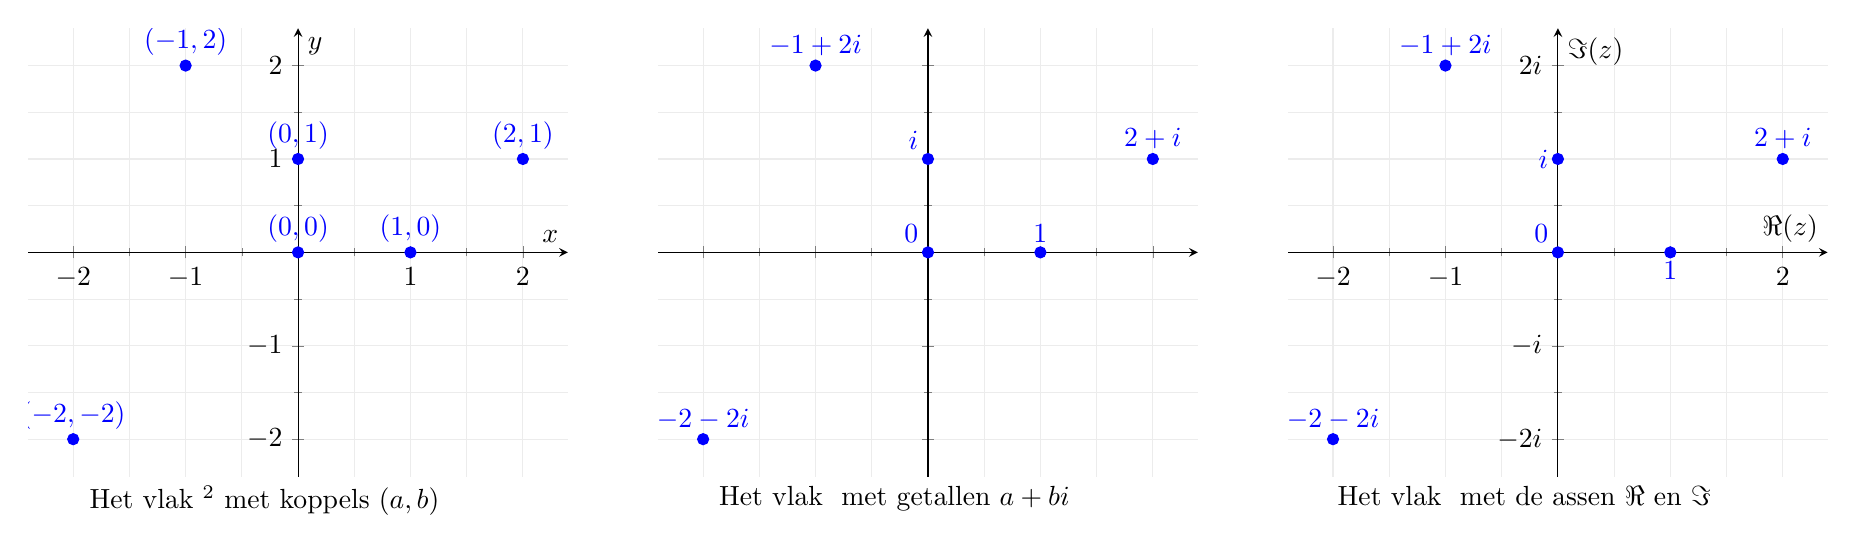
\begin{tikzpicture}[scale=1]	
			\begin{scope}[xshift=-8cm]
				\begin{axis}[
					axis lines = center,
					grid=both,
					grid style={gray!15},
					minor tick num=1,
					% ticks=both,
					xlabel=$x$,
					ylabel=$y$,
					ytick ={-7,...,8}, 
					xtick ={-7,...,8}, 
					ymin=-2,ymax=+2,
					xmin=-2,xmax=+2,
					enlargelimits=true,
					]
					
					\addplot [blue, mark = *] coordinates {( 0, 0)} node[above] {$(0,0)$};
					\addplot [blue, mark = *] coordinates {( 1, 0)} node[above] {$(1,0)$};
					\addplot [blue, mark = *] coordinates {( 0, 1)} node[above] {$(0,1)$};
					% \addplot [blue, mark = *] coordinates {( 2, 0)} node[above] {$(2,0)$};
					\addplot [blue, mark = *] coordinates {( 2, 1)} node[above] {$(2,1)$};
					\addplot [blue, mark = *] coordinates {( 2,-3)} node[above] {$(2,-3)$};
					\addplot [blue, mark = *] coordinates {(-1, 2)} node[above] {$(-1,2)$};
					\addplot [blue, mark = *] coordinates {(-2,-2)} node[above] {$(-2,-2)$};

				\end{axis}
				\node[below] at (3,0) {Het vlak $\R^2$ met koppels $(a,b)$};
			\end{scope}
	
			\begin{scope}[xshift=0cm]
				\begin{axis}[
					axis lines = center,
					grid=both,
					grid style={gray!15},
					minor tick num=1,
					% ticks=both,
					% xlabel=$\Re(z)$,
					% ylabel=$\Im(z)$,
					ytick ={-7,...,8}, yticklabels={},
					xtick ={-7,...,8}, xticklabels={},
					ymin=-2,ymax=+2,
					xmin=-2,xmax=+2,
					enlargelimits=true,
					]
					
					\addplot [blue, mark = *] coordinates {( 0, 0)} node[above left] {$0$};
					\addplot [blue, mark = *] coordinates {( 1, 0)} node[above     ] {$1$};
					\addplot [blue, mark = *] coordinates {( 0, 1)} node[above left] {$i$};
					% \addplot [blue, mark = *] coordinates {( 2, 0)} node[above left] {$2$};
					\addplot [blue, mark = *] coordinates {( 2, 1)} node[above] {$2+i$};
					\addplot [blue, mark = *] coordinates {( 2,-3)} node[above] {$2-3i$};
					\addplot [blue, mark = *] coordinates {(-1, 2)} node[above] {$-1+2i$};
					\addplot [blue, mark = *] coordinates {(-2,-2)} node[above] {$-2-2i$};
				\end{axis}
				\node[below] at (3,0) {Het vlak $\C$ met getallen $a+bi$};

			\end{scope}
	
			\begin{scope}[xshift=8cm]
				\begin{axis}[
					axis lines = center,
					grid=both,
					grid style={gray!15},
					minor tick num=1,
					% ticks=both,
					xlabel=$\Re(z)$,
					ylabel=$\Im(z)$,
					ytick ={-7,...,8}, yticklabels={$-7i$, $-6i$, $-5i$, $-4i$, $-3i$, $-2i$, $-i$, $0$, , $2i$, $3i$, $+3i$, $+4i$, $+5i$, $+6i$, $+7i$, $+8i$},
					xtick ={-3,...,3}, xticklabels={$-3$,$-2$,$-1$, , ,$2$,$3$},
					ymin=-2,ymax=+2,
					xmin=-2,xmax=+2,
					enlargelimits=true,
					]
					
					\addplot [blue, mark = *] coordinates {( 0, 0)} node[above left] {$0$};
					\addplot [blue, mark = *] coordinates {( 1, 0)} node[below] {$1$};
					\addplot [blue, mark = *] coordinates {( 0, 1)} node[left] {$i$};
					%\addplot [blue, mark = *] coordinates {( 2, 0)} node[above left] {$2$};
					\addplot [blue, mark = *] coordinates {( 2, 1)} node[above] {$2+i$};
					\addplot [blue, mark = *] coordinates {( 2,-3)} node[above] {$2-3i$};
					\addplot [blue, mark = *] coordinates {(-1, 2)} node[above] {$-1+2i$};
					\addplot [blue, mark = *] coordinates {(-2,-2)} node[above] {$-2-2i$};
				\end{axis}
				\node[below] at (3,0) {Het vlak $\C$ met de assen $\Re$ en $\Im$};
			\end{scope}
		\end{tikzpicture}
	\end{image}

	\begin{xmuitweiding}[Vermenigvuldigen met $i$ is draaien over $90\degree$]\nl
	We kunnen nu ook proberen deze nieuwe getallen met elkaar te vermenigvuldigen. 
	Als dat überhaupt mogelijk zou zijn, dan verwachten we zeker dat $i = 1\cdot i = i\cdot1$. 
	Dus, de actie 'vermenigvuldig met $i$' roteert $1$ (op de $x$-as) naar $i$ (op de $y$-as) over een hoek van $90\degree$in tegenwijzerzin.
	Als we zouden willen verkrijgen dat vermenigvuldigen met $i$ \textit{altijd} deze rotatie is over $90\degree$, dan moet $i$ vermenigvuldigd met $i$ landen op $-1$, want dat is waar je terechtkomt als je $i$ nog $90\degree$ verder roteert. Om van 'vermenigvuldig met $i$' een rotatie van $90\degree$ te maken moet dus zeker $i\cdot i=-1$. 
	Als we ook de gewone rekenregels zoals distributiviteit willen, dan ligt de vermenigvuldiging met $i$ nu volledig vast, want dan moet
	$$
	i\cdot(a+bi) = a\cdot i + b\cdot i\cdot i = ai + bi^2 = ai + b\cdot(-1) = ai - b = -b + ai.
	$$
	De wiskundige goden zijn ons goed gezind: het punt $(-b,a)$ is inderdaad ook het resultaat van een rotatie over $90\degree$ rond de oorsprong van het punt $(a,b)$, en we kunnen dus besluiten dat door $i^2=-1$ te stellen, we inderdaad bekomen dat het wat mysterieuze getal $i$ gewoon overeenkomt (bij vermenigvuldiging) met '$90\degree$ draaien in tegenwijzerzin'. Zeer mooi, zou je kunnen zeggen.
	\end{xmuitweiding}

	Als (bijna) gratis extra krijgen we bij deze nieuwe ziens- en schijfwijze een vermenigvuldiging cadeau. Het volstaat daarvoor om voor eens en voor altijd vast te leggen dat $i^2=-1$.

\begin{definition}\nl
	
Een \textbf{complex getal} is een uitdrukking $a+bi$, met $a,b \in \R$, en komt op unieke wijze overeen met het punt $(a,b)$ in het reële vlak $\R^2$.
Het nieuwe symbool $i$ noemt de \textbf{imaginaire eenheid}, en er geldt per definitie dat \important{i^2=-1}. 


\begin{image}[0.7\textwidth]
	\begin{tikzpicture}[scale=3]%,cap=round,transform canvas={scale=0.5}]
	
	\tikzmath{\hoek = 35;}
	
	\draw[->] (-0.1,0) -- (1.2,0) node[above] {Re$(z)$};
	\draw[->] (0,-0.1) -- (0,1)   node[right] {Im$(z)$};

	\draw[color=blue,thick] (0:0)  -- (\hoek:1); 
	%
	\draw[color=black] (\hoek:1) node[name=P,circle, fill=black, radius=1pt,scale=0.8] {} node [yshift=2pt,above] {$z=a+bi$} ;  
	%
	\draw[dashed] ({cos(\hoek)},0) node[circle, fill=black, radius=1pt,scale=0.5] {} node[below] {$a$} -- (P);
	\draw[dashed] (0,{sin(\hoek)}) node[circle, fill=black, radius=1pt,scale=0.5] {} node[left] {$bi$} -- (P);
	%
	\draw [thick, red,decorate,decoration={brace,amplitude=10pt,mirror},yshift=-5pt](0,0) -- ({cos(\hoek)},0) node[black,midway,yshift=-0.6cm] {\footnotesize $a$};
	%
	\draw [thick, red,decorate,decoration={brace,amplitude=10pt},xshift=-5pt](0,0) -- (0,{sin(\hoek)}) node[black,midway,left,xshift=-8pt] {\footnotesize $b$};
    
    \begin{scope}[xshift=-2cm]
    	\draw[->] (-0.1,0) -- (1.2,0) node[above] {$x$};
    	\draw[->] (0,-0.1) -- (0,1)   node[right] {$y$};
    
%    	\draw[color=blue,thick] (0:0)  -- (\hoek:1); 
    	%
    	\draw[color=black] (\hoek:1) node[name=P,circle, fill=black, radius=1pt,scale=0.8] {} node [yshift=2pt,above] {$(a,b)$} ;  
    	%
    	\draw[dashed] ({cos(\hoek)},0) node[circle, fill=black, radius=1pt,scale=0.5] {} node[below] {$a$} -- (P);
    	\draw[dashed] (0,{sin(\hoek)}) node[circle, fill=black, radius=1pt,scale=0.5] {} node[left] {$b$} -- (P);
    	%
    	\draw [thick, red,decorate,decoration={brace,amplitude=10pt,mirror},yshift=-5pt](0,0) -- ({cos(\hoek)},0) node[black,midway,yshift=-0.6cm] {\footnotesize $a$};
    	%
    	\draw [thick, red,decorate,decoration={brace,amplitude=10pt},xshift=-5pt](0,0) -- (0,{sin(\hoek)}) node[black,midway,left,xshift=-8pt] {\footnotesize $b$};
    \end{scope}
	
	\end{tikzpicture}
\end{image}

De verzameling van alle complexe getallen noteren we $\important{\C} = \{ a+bi | a,b\in\R; \ i^2=-1\}$.

Een willekeurig complex getal wordt dikwijls genoteerd met $z$. Als $z=a+bi$, spreken we niet langer over $x$- en $y$-coördinaat maar dan
\begin{itemize}
\item is $a$ het \textbf{reëel deel} van $z$, genoteerd als $\text{Re}(z) \perdef a$.
\item is $b$ het \textbf{imaginair deel} van $z$, genoteerd als $\text{Im}(z)\perdef b$.
\item Als $b=0$, dan is $z=a$ een \textbf{(zuiver) re\"eel getal} (en $\R$ is dus een deelverzameling van $\C$).
\item Als $a=0$, dan is $z=bi$ een \textbf{(zuiver) imaginair getal}. 
%We noteren de verzameling van die getallen soms als $i\R$.
\end{itemize}
\end{definition}


Twee complexe getallen $z$ en $w$  zijn dus aan elkaar gelijk zodra ze  dezelfde reële delen hebben, en dezelfde imaginaire delen:
$$
    z = w \quad \iff  \quad \Re(z)=\Re(w) \Ten \Im(z)=\Im(w).
$$


\begin{example} Volgende uitdrukkingen zijn allemaal complexe getallen:
$$
\def\arraystretch{1.5}
\begin{array}{c|rr c lll}
    z & \Re(z) & \Im(z) \\\hline
    2+3i & 2 & \answer{3} 
    \\
    5-6i &\answer{5} & \answer{-6} 
    \\
    1+i\sqrt{2} & 1 & \sqrt{2}
    \\
    \dfrac{1-i\sqrt{5}}{2}  & \dfrac{1}{2} & -\dfrac{\sqrt{5}}{2}
    \\
\end{array}
\qquad\qquad
\begin{array}{c|rr c lll}
    z & \Re(z) & \Im(z) \\\hline
    1+\pi & 1+\pi & 0
    \\
    42 & \answer{42} & 0
    \\
    42i & \answer{0} & \answer{42} 
    \\
    5i + 7 & \answer{7} & \answer{5} 
    \\
    2+ 5i + \pi & \answer{2+\pi} & \answer{5} 
    \\
\end{array}
$$
De getallen $42$ en $1+\pi$ zijn zuiver reële getallen, en $42i$ is een zuiver imaginair getal. 
\\
Van het complex getal $2+3i$ is het reëel deel $2$ en het imaginair deel $3$. 
\end{example}



Als we het vlak op deze manier bekijken als de verzameling van de complexe getallen, spreken we van het \textbf{complexe vlak}. Het getal $i$ komt daarbij overeen met het koppel $(0,1)$ op de $y$-as.

\begin{xmuitweiding}[Meetkundige betekenis van complexe getallen]\nl

	Volgende video legt kort uit hoe complexe getallen meetkundig worden voorgesteld.

\youtube{Ho_oadFkm1o}  % Bron: SPOC Complexe getallen


Volgende video legt in detail uit hoe complexe getallen \textit{meetkundig} kunnen worden voorgesteld.
In het bijzonder wordt de meetkundige interpretatie gegeven voor de vermenigvuldiging met $i$ uitgelegd.

% Uit de SPOC Complexe Getallen
\youtube{i1aPI3_nia4}

\end{xmuitweiding}

\end{document}

